\chapter{GCG}
% 1 Seite

	\begin{figure}[ht!]
		\centering
		\includesvg{Bilder/DrawIO/detection_overview}
		\caption{A simplified overview of the four major stages of solving a model with \acs{GCG}.}
		\label{fig:gcg:overview}
	\end{figure}

	In this chapter, we introduce \acf{GCG}, a decomposition solver which is based on the open-source MIP-Solver \ac{SCIP} \cite{gamrathExperimentsGenericDantzigWolfe2010}.
	Readers already experienced with GCG and its capabilities may still find some details and observations interesting.
	For a given problem, \acs{GCG} is able to perform an automatic Dantzig-Wolfe reformulation which is then solved using a branch-price-and-cut algorithm.
	Alternatively, \ac{GCG} support a special \textit{Benders-Mode} which reformulated the problem using Benders decomposition.
	
	In contrast to other open-source solvers like \acfreverse{BaPCod} \cite{sadykovBaPCodGenericBranchandprice2021} or commercial software such as \textit{SAS} \cite{SASDataAI} which rely solely on user-provided decompositions, \ac{GCG} is able to automatically detect different kinds of structures algorithmically, including but not limited to
	\begin{itemize}
		\item Single-Bordered structures
		\item Arrowhead structures using the third-party tool \acfreverse{hMETIS} \cite{karypisMultilevelHypergraphPartitioning1997}.
		\item Staircase structures
	\end{itemize}
	\todo{Entfernen und auf Kapitel vorher ref}
	
	The solving process in divided into multiple consecutive stages as shown in Figure \ref{fig:gcg:overview}. Each stage will be explained in more detail in the following section as needed.
	The detection in particular aims to make \ac{GCG} more accessible to a wider range of users which do not necessarily have the required theoretical background and practical experience to reformulate linear programs on their own.
	For more details about individual features and capabilities, we refer to the official documentation \cite{GCG}. \todo{Kurz die 4 Schritte aus Bild erwähnen und einen Satz}

	\section{Detection}
	% 2 Seiten, Detection Loop etc.
	
		\begin{figure}[ht!]
			\centering
			\includesvg[scale=0.73]{Bilder/DrawIO/detection_loop}
			\caption{A simplified overview of the detection process and its detection loop.}
			\label{fig:gcg:detectionloop}
		\end{figure}
	
		As mentioned in the introduction to this chapter, one integral part and distinguishing feature of \ac{GCG} is its detection framework.
		A simplified overview of the detection currently \footnote{\ac{GCG} version 3.5, as of 2025-07-18.} implemented in \ac{GCG} is shown in Figure \ref{fig:gcg:detectionloop}. For a more detailed visualization including additional information about how pre-solving is handled we refer to the official documentation \cite{GCG}.
		The framework consists of two major parts:
		
		\begin{enumerate}
			\item A \textbf{classification} step, in which a set of classifiers is partitioning the constraints (and variables) according to a certain property, producing one partition each.
			The goal of this step is to detect different underlying structures of the constraint matrix, which can be used during the detection loop to make more informed decisions about which constraints to assign to which block or master.
			Important classifiers for the remainder of this thesis are discussed in more detail in Section \ref{chap:gcg:classifiers}.
			\item The \textbf{detection loop}, which consists of a set of detectors which are responsible for assigning constraints either the master or to individual blocks.
			In round $n+1$ a detector receives a \textit{partial} decomposition, that is, a decomposition in which \textit{not all} constraints are assigned yet, from round $n$ as input and pushes a set of newly created (partial) decompositions to a queue.
			In case the user did not provide a partial decomposition as input in round $0$, the loop is initialized with a decomposition in which no constraint is assigned yet.
		\end{enumerate}
	
		\begin{figure}[ht!]
			\centering
			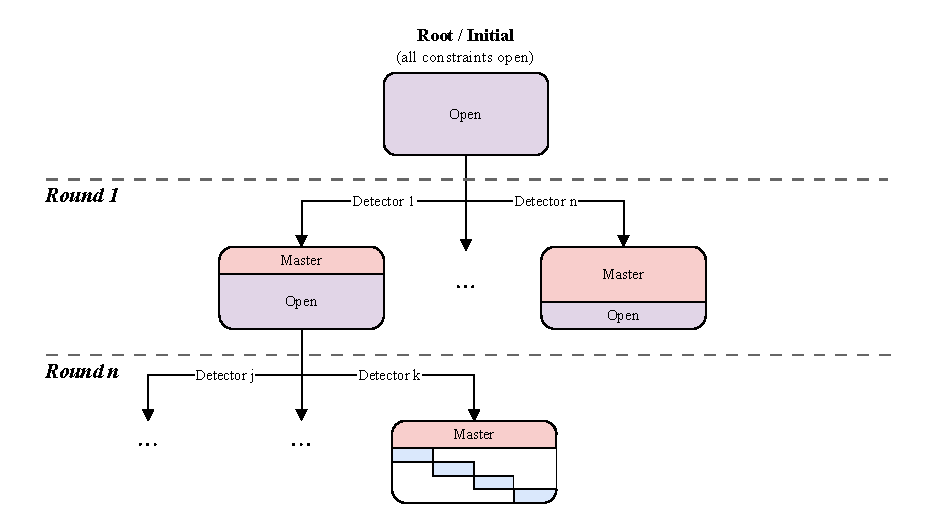
\includegraphics{Bilder/DrawIO/partialdec_tree_pdf}
			\caption{Visualization of the induced tree of propagated partial decompositions.}
			\label{fig:gcg:partialdettree}
		\end{figure}
		
		The concept of detecting structures in different rounds is visualized in Figure \ref{fig:gcg:partialdettree}.
		Starting from a root decomposition in which all constraints are still unassigned or \enquote{open}, different detectors produce a set of new partial decomposition.
		Depending on the configuration, a detector is not allowed to work on a certain partial decomposition or its decedents twice.
		A very simple but concrete example of how such a tree might look like in practice can be found in Section \ref{chap:gcg:example}.
		
		Furthermore, if no detector found any new decomposition in round $k$, or $k$ exceed the maximum number of rounds, the detection loop is stopped and all complete decomposition are collected, scored and exactly one is chosen for which the solving is started. \todo{Grammatik, Wortwahl}
		The scoring and selection stage is of particular interest in practice, because the tree in Figure \ref{fig:gcg:partialdettree} might grow beyond thousand of decompositions, of which the best in terms of solving time or a different metric must be selected.
		Because the scoring of decompositions is not of major interest for \textit{this} thesis, we refer to the official documentation for details \cite{GCG}.
	
	\clearpage
	
	\section{Classifiers}
	\label{chap:gcg:classifiers}
		% 1 Seite, Var Classifiers
		% 1 Seite, Cons Classifiers
		
		\subsection{Name Classifiers}
		
			
		
		\subsection{Numeric Classifiers}
		
			In contrast to a classifier based on properties the  lassifiers are solely based on 
		
			\clearpage
		
		\subsection{Type Classifiers}
		
			Classifiers based 
			
			\subsubsection{SCIP Types}
			
				When using \ac{GCG} as a library, the type of a variable or constraint can be retrieved via. \lstinline|SCIPconsGetType(cons)| or \lstinline|SCIPvarGetType(cons)| respectively.
				The former function is not provided by \ac{SCIP} itself, but is implemented in \ac{GCG} instead.
				The implementation compares the name of the handler the constraint is assigned to and compares it to a known list of constraint handlers. \todo{the}
				The list of supported handlers includes \emph{Knapsack}, \emph{Set Partitioning}, \emph{Set Covering}, \emph{Set Packing}, \emph{Varbound} and \emph{General}, in case no special structure was detected. \todo{Check List}
				Variables can be classified as \emph{Integer}, \emph{Binary} or \emph{Continuous}
				\footnote{There are more types of variables in newer versions of \ac{SCIP} such as \emph{Implicit Integer}, but these three basic types are sufficient for the purpose of this discussion.}.
				
				The clear downside of this classification is its important precondition.
				In order to use this feature properly and retrieve a meaningful type via. the two methods, pre-solving must have been executed prior to detection.
				When \ac{GCG} reads the problem as e.g. an \lstinline|.lp| file, all constraints are added as linear constraints to the underlying \ac{SCIP} model.
				These constraints are usually \enquote{upgraded} if possible, that is, their structure is analyzed and assigned to the correct constraint handler during pre-solving.
				This is done to take advantage of properties only possessed by certain types of constraints, e.g. a solution to a set of Knapsack constraints \textit{can} be computed more efficiently by using an algorithm based on dynamic programming.
				For more detailed information we refer to the official documentation \cite{SCIPDoxygenDocumentation}.
				
				Preliminary testing showed that it is not trivial to configure the pre-processing in such a way that \textit{only} the upgrade mechanism is triggered and variables and constraints remain unchanged. \todo{Add test config to appendix}
				
				\clearpage
		
			\subsubsection{MIPLIB Constraint Types}
			
				\begin{table}[ht!]
					\centering
					\begin{tabular}{l|l|l|l}
						\textbf{Nr.} & \textbf{Type} & \textbf{Linear Constraint} & \textbf{Notes} \\
						\hline
						\hline
						1 & Empty & $\emptyset$ & - \\
						2 & Free & $-\infty \leq x \leq \infty$ & No finite side. \\
						3 & Singleton & $a \leq x \leq b$ & - \\
						4 & Aggregation & $ax + by = c$ & - \\
						5 & Precedence & $ax - ay \leq b$ & $x$, $y$ have same type. \\
						6 & Variable Bound & $ax + by \leq c$ & $x \in \{0, 1\}$ \\
						7 & Set Partitioning & $\sum 1 x_i = 1$ & $\forall i: x_i \in \{0, 1\}$ \\
						8 & Set Packing & $\sum 1 x_i \leq 1$ & $\forall i: x_i \in \{0, 1\}$ \\
						9 & Set Covering & $\sum 1 x_i \geq 1$ & $\forall i: x_i \in \{0, 1\}$ \\
						10 & Cardinality & $\sum 1 x_i = b$ & $\forall i: x_i \in \{0, 1\}, b \in \mathbb{N}_{\geq 2}$ \\
						11 & Invariant Knapsack & $\sum 1 x_i \leq b$ & $\forall i: x_i \in \{0, 1\}, b \in \mathbb{N}_{\geq 2}$ \\
						12 & Equation Knapsack & $\sum a_i x_i = 1$ & $\forall i: x_i \in \{0, 1\}, b \in \mathbb{N}_{\geq 2}$ \\
						13 & Bin Packing & $\sum a_i x_i + ay \leq a$ & $\forall i: x_i, y \in \{0, 1\}, b \in \mathbb{N}_{\geq 2}$ \\
						14 & Knapsack & $\sum a_i x_i \leq b$ & $\forall i: x_i \in \{0, 1\}, b \in \mathbb{N}_{\geq 2}$ \\
						15 & Integer Knapsack & $\sum a_i x_i \leq b$ & $\forall i: x_i \in \mathbb{Z}, b \in \mathbb{N}$ \\
						16 & Mixed Binary & $\sum a_i x_i + \sum p_j s_j \; \{\leq, =\} \; b$ & $\forall i: x_i \in \{0, 1\}, \forall j: s_j \; \mathrm{continuous}$ \\
						17 & General Linear & $\sum a_i x_i \; \{\leq, \geq, =\} \; b$ & No special structure.
					\end{tabular}
					\caption{The structure of all 17 constraint types MIPLIB keeps track of.}
					\label{table:constypes:miplib}
				\end{table}
				
				In order to get a more fine-grained classification based on inferred constraint types, 
		\clearpage
		
	\subsection{Detectors}
	% 1 Seite
	
	\section{Existing Detectors}
	% 1 Seite, trivial Detectors
	% 1 Seite, HMETIS Detectors
	% 1 Seite , other Detectors
	
	\section{Example}
	\label{chap:gcg:example}
	
		\begin{figure}[ht!]
			\centering
			\begin{align*}
				&\min &\sum_{j=1}^m y_j \\
				&\text{s.t.} &\sum_{j=1}^m x_{ij} &= 1 &&\forall i \in \mathcal{I} \\
				&& \sum_{i=1}^n a_i x_{ij} &\leq C y_j && \forall j \in \mathcal{J} \\
				&& x_{ij} &\in { 0, 1} && \forall i \in \mathcal{I}, \forall j \in \mathcal{J} \\
				&& y_j &\in { 0, 1 } && \forall j \in \mathcal{J}
			\end{align*}
			\caption{Bin-Packing Model with items $\mathcal{I} = \{ 1, \ldots, n \}$, item sizes $a_i \in \mathbb{Z}_{\geq 0}$, bins $\mathcal{J} = \{ 1, \ldots, m \}$ and capacity $C$.}
			\label{figure:gcg:example:binpack}
		\end{figure}
		
		In order to illustrate the detection 
		
		